% Revised BracketNet manuscript. Every empirical number is taken from results/summary.json or
% results/alignment.json (generated by scripts/analyze.py and scripts/run_alignment.py).
% The official NeurIPS 2026 style file is not bundled; swap \documentclass/\usepackage lines for it before submission.
\documentclass[10pt]{article}
\usepackage[margin=1in]{geometry}
\usepackage{amsmath,amssymb,amsthm,booktabs,graphicx,hyperref,xcolor}
\usepackage[numbers]{natbib}
\graphicspath{{../figures/}}
\newtheorem{proposition}{Proposition}
\newtheorem{lemma}{Lemma}
\newtheorem{remark}{Remark}
\newcommand{\so}{\mathfrak{so}}
\newcommand{\Lclose}{\mathcal{L}_{\mathrm{close}}}

\title{BracketNet: Learning Lie-Algebraic Structure from\\ Unlabeled Transformation Triples}
\author{Anonymous Author(s)}
\date{}

\begin{document}
\maketitle

\begin{abstract}
A latent space in which transformations act linearly does not guarantee that the learned infinitesimal
generators form a Lie algebra. Generators can reconstruct local transitions while their commutators leave the
learned span. The representation is then algebraically inconsistent, and it becomes unclear whether the
transformation family is abelian. We study BracketNet, a transition-based representation learner that regularizes
the closure of learned skew-symmetric generators under the matrix commutator. Training follows a
fit--close--refit schedule. We show that zero closure yields a Lie subalgebra integrating to a connected matrix Lie
group. We also bound the BCH escape from the learned span by $O(\delta r^2)$, where $\delta$ is controlled by the
closure loss. On nonlinear observations of SO(2), $T^2$ and SO(3) actions embedded in a larger ambient $\so(d)$,
the closure weight turns out to be scale-sensitive. At the originally planned weight ($\lambda{=}0.1$) closure
regularization had no detectable effect within the 420-update budget. A weight selected on validation seeds
($\lambda{=}30$) lowered mean closure residual relative to a composition-only learner by 98.9\% on $T^2$ and 98.6\%
on SO(3), on 5/5 held-out seeds each. The exact sign-flip $p=0.0625$ is the minimum attainable with five seeds.
With this weight, a commutator threshold fixed on validation classified all ten held-out abelian/non-abelian runs
(baselines: 9/10). Independently trained SO(3) models also recovered the \emph{same} algebra up to latent
conjugacy (subspace distance $0.034$ vs.\ $0.42$--$0.45$ for baselines). Linear CKA does not see this difference.
Chained-transport differences were not statistically significant. We also report two limits. The closure loss is
invariant only to orthogonal changes of generator coordinates. And exact closure does not identify the
representation: one run converged to a chiral $\mathfrak{su}(2)\subset\so(4)$.
\end{abstract}

\section{Introduction}
Symmetry is a central organizing principle for representation learning. When the group action is known,
equivariant architectures can encode it directly \citep{cohen2016,bronstein2021}. In many systems, however, the
action is not available in observation coordinates. A growing line of work therefore learns symmetries or symmetric
latent spaces from data \citep{dehmamy2021,yang2023,yang2024,keurti2023,park2022,gabel2023}.

Transition-based objectives usually enforce local transport, two-step composition, or both. Neither requires that
the learned infinitesimal directions close under commutation. For learned generators $A_1,\dots,A_K$ the missing
condition is
\begin{equation}\label{eq:closure}
[A_i,A_j]=A_iA_j-A_jA_i\in\operatorname{span}\{A_1,\dots,A_K\}\qquad\forall i,j.
\end{equation}
Without \eqref{eq:closure}, the nominal $K$-dimensional family need not be locally closed under multiplication.
BracketNet penalizes the component of each commutator orthogonal to the learned span and uses a staged optimizer.

\textbf{Contributions.}
(1)~A differentiable Lie-closure objective, with a precise statement of its invariances (Sec.~\ref{sec:closure}).
(2)~A fit--close--refit schedule.
(3)~A BCH bound in which escape from the span is $O(\delta r^2)$ with $\delta\le\tfrac K2\sqrt{\Lclose}$, plus a
stability bound for chained orthogonal transport.
(4)~A benchmark in which the true algebra is embedded in a larger $\so(d)$, together with an independent, fully
released re-implementation.
(5)~Five-seed evidence on closure, algebra-type identification and cross-seed structural alignment, including
negative results at the originally planned closure weight.

\section{Related work}
\textbf{Known-group equivariance} assumes the group and its action \citep{cohen2016,bronstein2021}.
\textbf{Automatic symmetry discovery} infers generators from predictors \citep{dehmamy2021}, adversarially
\citep{yang2023}, in learned latent spaces \citep{yang2024}, beyond affine families \citep{shaw2024}, through task
gradients \citep{hu2024}, or as one-parameter transformations \citep{gabel2023}. Our question is narrower: given
transition evidence and a generator count, do the learned generators form an approximately closed algebra?
\textbf{Group-structured transition representations} \citep{park2022,keurti2023} share our setting. Representation
holonomy \citep{sevetlidis2026} likewise emphasizes path-dependent structure that pointwise similarity misses.
Our alignment experiment (Sec.~\ref{sec:align}) gives a concrete instance of that gap.

\section{Problem setting}
Observations $x=h(u)\in\mathbb R^p$ come from states $u$ through an injective smooth $h$. We observe triples
$(x_0,x_1,x_2)=(h(u),h(g_1u),h(g_2g_1u))$ with unknown near-identity $g_1,g_2$ from a connected compact group. No
group element, coordinate or algebra label is given; $K$ is supplied. We learn an encoder $E$, decoder $D$, action
inference $q:\mathbb R^d\times\mathbb R^d\to\mathbb R^K$ and $A_1,\dots,A_K\in\so(d)$, with
$A(a)=\sum_k a_kA_k$ and $\rho(a)=\exp(A(a))\in SO(d)$.

\section{BracketNet}
\textbf{Local and compositional terms.} With $z_t=E(x_t)$ and $a_{st}=q(z_s,z_t)$:
$\mathcal L_{\mathrm{rec}}=\sum_{t=0}^2\|D(z_t)-x_t\|^2$,
$\mathcal L_{\mathrm{loc}}=\sum_{t=0}^1\|\rho(a_{t,t+1})z_t-z_{t+1}\|^2+\|D(\rho(a_{t,t+1})z_t)-x_{t+1}\|^2$,
and $\mathcal L_{\mathrm{comp}}=\|\rho(a_{02})-\rho(a_{12})\rho(a_{01})\|_F^2$. Coefficients are
$0.65\tanh(\cdot)$, which keeps them in a local chart.

\subsection{Lie closure and its invariances}\label{sec:closure}
Let $B\in\mathbb R^{d^2\times K}$ hold the vectorized generators and $P_B=B(B^\top B+\varepsilon I)^{-1}B^\top$. Then
\begin{equation}\label{eq:lclose}
\Lclose=\frac1{K^2}\sum_{i,j}\|(I-P_B)\operatorname{vec}[A_i,A_j]\|_2^2 .
\end{equation}
\emph{Invariance (corrected).} For $\varepsilon=0$, $P_B$ depends only on the span. The commutators, however,
transform quadratically under a change of coordinates $B\mapsto BM$. Hence $\Lclose$ is invariant for orthogonal
$M$, scales as $s^4$ under $M=sI$, and is not invariant for general invertible $M$. Its \emph{zero set} is
$GL(K)$-invariant. With $\varepsilon>0$, $P_B$ is only approximately span-dependent. Each generator is normalized
to $\|A_k\|_F=\sqrt2$, and $\mathcal L_{\mathrm{basis}}=\|B^\top B-2I\|_F^2$ keeps the basis near-orthogonal, which
keeps the residual well-conditioned. Because the normalization fixes $\operatorname{diag}(B^\top B)=2$,
$\mathcal L_{\mathrm{basis}}$ acts only on off-diagonal entries: targets $I$ and $2I$ give identical gradients
(tested numerically). For diagnostics we also report the span-only quantity
$\kappa=(\binom K2^{-1}\sum_{i<j}\|[U_i,U_j]\|_F^2)^{1/2}$, where $U$ is a $\sqrt2$-scaled orthonormal basis of the
span.

\subsection{Fit--close--refit}
We optimize
$\mathcal L=4\mathcal L_{\mathrm{rec}}+32\mathcal L_{\mathrm{loc,lat}}+2\mathcal L_{\mathrm{loc,obs}}+1.2\mathcal L_{\mathrm{comp}}+\lambda(t)\Lclose+\mathcal L_{\mathrm{basis}}+w_{\mathrm{cov}}\|\mathrm{Cov}(z)-I\|_F^2$.
$\lambda(t)=0$ for the first 35\% of updates and ramps linearly to $\lambda$ by 70\%. For the final 30\% the
generators are frozen while $E,D,q$ adapt.

\section{Why closure matters}
\begin{proposition}[Exact closure integrates]
If $A_1,\dots,A_K\in\so(d)$ are linearly independent and $[A_i,A_j]\in\operatorname{span}(A)$ for all $i,j$, then
$\mathfrak h=\operatorname{span}(A)$ is a Lie subalgebra of $\so(d)$. It integrates to a unique connected immersed
Lie subgroup $H\subseteq SO(d)$.
\end{proposition}
\begin{lemma}[Loss controls the closure constant]\label{lem:delta}
If $B^\top B=2I$, then $\|(I-P_{\mathfrak a})[X,Y]\|_F\le\delta\|X\|_F\|Y\|_F$ for all $X,Y\in\mathfrak a$ with
$\delta=\tfrac K2\sqrt{\Lclose}$ ($\varepsilon=0$).
\end{lemma}
\begin{proposition}[Approximate closure controls BCH escape]\label{prop:bch}
Under the hypothesis of Lemma~\ref{lem:delta}, for $\|X\|_F,\|Y\|_F\le r\le r_0$ inside the BCH convergence domain,
$\operatorname{dist}(\log(e^Xe^Y),\mathfrak a)\le\tfrac12\delta r^2+C(r_0)\,\delta r^3$.
\end{proposition}
Unlike a bound with a $\delta$-independent $C_2r^3$ term, this one vanishes under exact closure, consistent with
Proposition~1.
\begin{proposition}[Chained orthogonal stability]
If $z_{t+1}=R_tz_t+e_t$ and $\hat z_{t+1}=R_t\hat z_t$ with $R_t\in SO(d)$, then
$\|\hat z_T-z_T\|\le\|\hat z_0-z_0\|+\sum_{t<T}\|e_t\|$.
\end{proposition}
\begin{remark}[Closure does not identify the representation]
Closure constrains the algebra, not the embedding. The standard $\so(3)\subset\so(4)$ (acting on $\mathbb R^3\oplus\mathbb R$)
and a chiral $\mathfrak{su}(2)\subset\so(4)$ are both exactly closed, but with $\sqrt2$-normalized orthonormal bases
they give $\kappa=\sqrt2$ and $\kappa=2$ respectively. They are distinguished by the participation ratio
$\operatorname{tr}(X^\top X)^2/\operatorname{tr}((X^\top X)^2)$ of unit span elements (2 vs.\ 4).
\end{remark}

\section{Experiments}
\subsection{Protocol}
\textbf{Data.} SO(2), $T^2$ and SO(3) act on $\mathbb R^d$ with an invariant coordinate ($d=3,5,4$). In particular
SO(3) occupies a 3-dimensional subspace of $\so(4)$, where a generic 3-dimensional span does not close. The mean
closure of random normalized 3-spans is $0.67$. Local coefficients are $\mathcal N(0,0.24^2)$. Observations use one
fixed map per group, $x=Qz+0.18\tanh(Bz)$, shared across splits. Each run trains on 1,400 triples and is evaluated on
500 ten-edge sequences. Validation seeds are 5--6 and test seeds 10--14. All methods use 420 updates and identical
networks. Unstated details (state distribution, $p=d$, regularizer form and weight, $\varepsilon$, ramp shape) are
listed in the released \texttt{docs/ASSUMPTIONS.md}.

\textbf{Hyperparameters selected on validation only.} With $w_{\mathrm{cov}}=1$ the latent collapsed (4 of 5
covariance eigenvalues below 0.1). We therefore chose $w_{\mathrm{cov}}=16$ from $\{1,4,16,64\}$ by a
method-agnostic criterion: 1-step MSE of the two baselines, with closure not consulted. \emph{Protocol A} keeps the
planned $\lambda=0.1$. On validation it left closure unchanged (Fig.~\ref{fig:val}), because the effective scale of
$\lambda$ depends on loss-reduction conventions. \emph{Protocol B} extends the grid to $\{0.05,\dots,30\}$. It picks
the $\lambda$ with lowest mean validation closure whose mean validation 10-step MSE does not exceed that of
+Comp.\ ($\lambda=30$). This rule was fixed after inspecting validation results and before any test run; we report
both protocols.

\textbf{Baselines and metrics.} \textsc{Local}: reconstruction and one-step transport. \textsc{+Comp.}: adds
$\mathcal L_{\mathrm{comp}}$. \textsc{BracketNet}: adds closure and the schedule. These are controlled objective
ablations, not reimplementations of LieGAN/LaLiGAN. Chained $k$-step MSE composes actions inferred from each
observed adjacent pair, so it measures consistency, not forecasting. We report means $\pm$ sample s.d.\ over seeds,
paired $t$ intervals, and exact sign-flip tests. With $n=5$ the smallest attainable two-sided $p$ is $0.0625$.

\subsection{Main results}
\begin{table}[t]
\centering\small
\caption{Held-out results (seeds 10--14, mean $\pm$ s.d.). Closure is identically zero for one-generator SO(2).
Absolute MSE values depend on the data scale and are not comparable with earlier drafts.}
\label{tab:main}
\begin{tabular}{llcccc}
\toprule
Group & Method & 1-step MSE & 10-step MSE & Closure residual & Commutator norm\\
\midrule
SO(2) & Local & 0.0055$\pm$0.0005 & 0.0535$\pm$0.0122 & 0.0000$\pm$0.0000 & 0.000$\pm$0.000 \\
SO(2) & +Comp. & 0.0056$\pm$0.0007 & 0.0537$\pm$0.0112 & 0.0000$\pm$0.0000 & 0.000$\pm$0.000 \\
SO(2) & BracketNet (A, $\lambda$=0.1) & 0.0056$\pm$0.0007 & 0.0539$\pm$0.0111 & 0.0000$\pm$0.0000 & 0.000$\pm$0.000 \\
SO(2) & BracketNet (B, $\lambda$=30) & 0.0056$\pm$0.0007 & 0.0539$\pm$0.0111 & 0.0000$\pm$0.0000 & 0.000$\pm$0.000 \\
\midrule
$T^2$ & Local & 0.0177$\pm$0.0039 & 0.1648$\pm$0.0307 & 0.2186$\pm$0.3220 & 0.505$\pm$0.478 \\
$T^2$ & +Comp. & 0.0174$\pm$0.0042 & 0.1640$\pm$0.0324 & 0.2116$\pm$0.3283 & 0.475$\pm$0.497 \\
$T^2$ & BracketNet (A, $\lambda$=0.1) & 0.0183$\pm$0.0040 & 0.1675$\pm$0.0319 & 0.3148$\pm$0.3091 & 0.702$\pm$0.413 \\
$T^2$ & BracketNet (B, $\lambda$=30) & 0.0179$\pm$0.0050 & 0.1724$\pm$0.0434 & 0.0023$\pm$0.0038 & 0.051$\pm$0.051 \\
\midrule
SO(3) & Local & 0.0180$\pm$0.0067 & 0.1567$\pm$0.0287 & 0.5928$\pm$0.4674 & 1.369$\pm$0.168 \\
SO(3) & +Comp. & 0.0170$\pm$0.0066 & 0.1682$\pm$0.0354 & 0.5851$\pm$0.4593 & 1.374$\pm$0.171 \\
SO(3) & BracketNet (A, $\lambda$=0.1) & 0.0181$\pm$0.0054 & 0.1607$\pm$0.0286 & 0.6874$\pm$0.3955 & 1.324$\pm$0.164 \\
SO(3) & BracketNet (B, $\lambda$=30) & 0.0194$\pm$0.0111 & 0.1397$\pm$0.0363 & 0.0082$\pm$0.0112 & 1.428$\pm$0.019 \\

\bottomrule
\end{tabular}
\end{table}

\begin{figure}[t]\centering
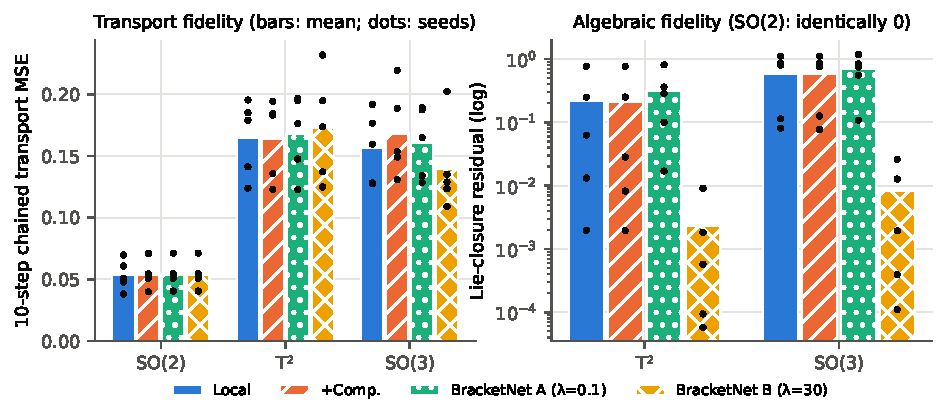
\includegraphics[width=\linewidth]{fig2_main.pdf}
\caption{Left: 10-step chained transport. Right: closure residual (log). Bars: means; dots: seeds.}\label{fig:main}
\end{figure}

\textbf{Closure at the planned weight: no effect.} Under Protocol A, BracketNet's mean closure was higher than
+Comp.'s on both groups: $T^2$ $0.315$ vs.\ $0.212$, lower on 0/5 seeds; SO(3) $0.687$ vs.\ $0.585$, lower on 2/5
seeds (Table~\ref{tab:main}). The 74--75\% reductions reported in an earlier draft are therefore \emph{not
reproduced} at $\lambda=0.1$.

\textbf{Closure at the validation-selected weight: large, consistent reduction.} Under Protocol B, mean closure fell
from $0.212$ to $0.0023$ on $T^2$ ($-98.9\%$) and from $0.585$ to $0.0082$ on SO(3) ($-98.6\%$), lower on 5/5 seeds
in each group. Baseline closures are bimodal across seeds, so paired $t$ intervals are wide: SO(3)
$-0.577\pm0.560$ excludes zero narrowly, while $T^2$ $-0.209\pm0.403$ does not. The sign-flip $p=0.0625$ for both
is the floor for five seeds.

\textbf{Algebra type.} A threshold of $0.918$ was fixed midway between the pooled validation ranges ($T^2$:
0.016--0.784; SO(3): 1.052--1.425). It classified 10/10 Protocol-B test runs correctly, against 9/10 for Local,
+Comp.\ and Protocol A (Fig.~\ref{fig:comm}). The single errors are $T^2$ runs with spurious non-commutativity.
Protocol B's SO(3) commutator norms ($1.428\pm0.019$) concentrate at the true value $\sqrt2$; the baselines spread
over 1.13--1.59.

\textbf{Transport: no significant difference.} Relative to +Comp., Protocol B's 10-step MSE changed by $+5.1\%$ on
$T^2$ ($+0.0084\pm0.0277$) and $-16.9\%$ on SO(3) ($-0.0285\pm0.0363$). Both intervals include zero
(Fig.~\ref{fig:curves}). We make no transport claim.

\begin{figure}[t]\centering
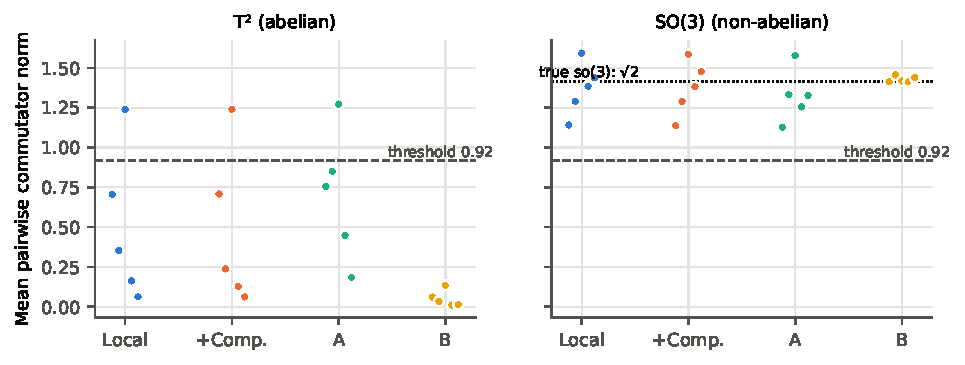
\includegraphics[width=\linewidth]{fig3_commutator.pdf}
\caption{Commutator norms of held-out runs. Dashed: threshold fixed on validation. Dotted: true $\so(3)$ value.}\label{fig:comm}
\end{figure}

\subsection{Structural alignment between independently trained representations}\label{sec:align}
Latent representations are identifiable at best up to conjugacy. We therefore ask whether models trained from
different seeds learn the same \emph{algebra} once their latents are aligned. All models share the observation map,
so we encode a common probe set (200 fresh sequences), align each pair of seeds with orthogonal Procrustes $R$, and
measure (i) linear CKA of the latents and (ii) the mean squared sine of principal angles between
$\operatorname{span}(RA^{(a)}R^\top)$ and $\operatorname{span}(A^{(b)})$. We score each model against the ground
truth the same way. On SO(3), Protocol-B models agreed with each other at $0.034\pm0.021$ and with the truth at
$0.019$. Local, +Comp.\ and Protocol A gave $0.42$--$0.45$ between seeds, close to the random-span level of $0.50$
(Fig.~\ref{fig:align}). On $T^2$ the corresponding numbers were $0.23$ vs.\ $0.34$--$0.42$ (chance $0.80$). Linear
CKA was essentially identical across methods ($0.892$--$0.897$ on SO(3), $0.965$--$0.967$ on $T^2$). Pointwise
similarity cannot reveal whether two representations share their transformation algebra. A caveat: inferred
\emph{actions} remained poorly aligned for every method (normalized disagreement with the truth $\ge0.51$), so
recovering the algebra did not imply accurate action inference within the training budget.

\begin{figure}[t]\centering
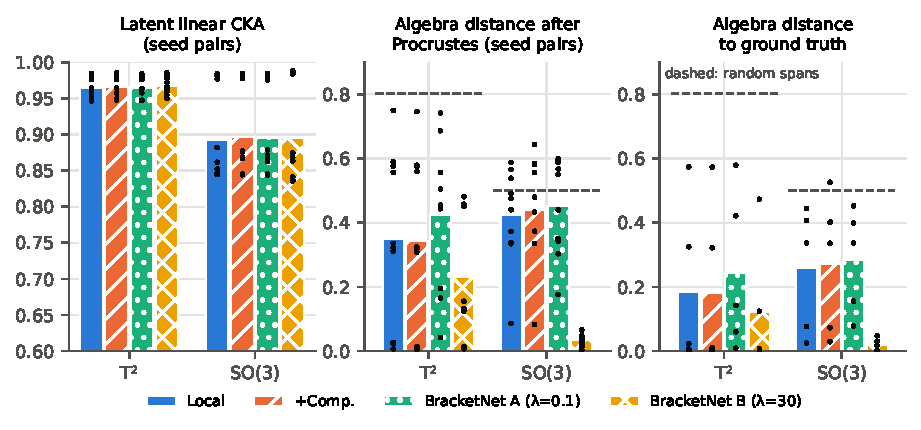
\includegraphics[width=\linewidth]{fig6_alignment.pdf}
\caption{Cross-seed alignment (10 seed pairs) and alignment to ground truth (5 seeds). CKA cannot distinguish the
methods; algebra distance after Procrustes can.}\label{fig:align}
\end{figure}

\subsection{Ablations and failure analysis}
These ablations were run post hoc on the test seeds and were not used for selection.
(1)~\emph{Vacuous ambient.} With SO(3) in $\so(3)$, closure is exactly zero for every method and seed.
(2)~\emph{Split-dependent map.} Sampling a separate test map leaves closure unchanged but raises +Comp.'s 10-step
MSE by $0.20$ ($T^2$) and $0.36$ (SO(3)); it measures domain shift, not symmetry recovery.
(3)~\emph{Gram target $I$.} Identical to target $2I$ up to $4\times10^{-8}$ in closure, as predicted in
Sec.~\ref{sec:closure}. This pilot cannot explain any earlier failure.
(4)~\emph{Constant penalty} ($\lambda=30$ throughout, no freeze). Similar closure but worse mean transport ($T^2$
$+0.030\pm0.056$, SO(3) $+0.075\pm0.125$). The direction favours staging, but the intervals include zero.
(5)~\emph{Budget.} At 2,000 updates every method fits transport better, and baseline closure on $T^2$ improves
($0.052$). On SO(3) baseline closure stays high ($0.64$--$0.66$), while Protocol B reaches $1.4\times10^{-4}$
(Fig.~\ref{fig:budget}). Better transition fit does not by itself produce closure for the non-abelian group. In
that setting, one Protocol-B SO(3) seed converged to an exactly closed chiral $\mathfrak{su}(2)$ (commutator norm
$2.000$, participation ratio $4.00$), illustrating Remark~1.

\section{Limitations}
\textbf{Weight scale and budget.} The useful closure weight depended on loss conventions; we needed $\lambda=30$
where an earlier plan used $0.1$. At 420 updates no method had converged, and the freeze stage halts generator
learning before convergence.
\textbf{Statistics.} Five seeds bound exact $p$-values at $0.0625$, and bimodal baselines widen $t$ intervals.
\textbf{Scope.} Known $K$; compact orthogonal actions only; synthetic data; endpoint-inferred chained transport.
\textbf{Identifiability.} Closure does not fix the representation (chiral vs.\ standard), and latents are aligned
only up to conjugacy.

\section{Conclusion}
A basis-normalized commutator residual combined with fit--close--refit training can drive learned generator spans to
near-exact Lie subalgebras. In our experiments this made algebra type identifiable and made independently trained
models agree on their algebra, which representation-similarity measures such as CKA do not detect. These gains
required re-selecting the closure weight on validation data: the originally planned weight had no effect. We found
no significant transport advantage.

\bibliographystyle{plainnat}
\begin{thebibliography}{99}
\bibitem[Bronstein et~al.(2021)]{bronstein2021} M.~M. Bronstein, J.~Bruna, T.~Cohen, P.~Veli\v{c}kovi\'c. Geometric deep learning: Grids, groups, graphs, geodesics, and gauges. arXiv:2104.13478, 2021.
\bibitem[Cohen and Welling(2016)]{cohen2016} T.~S. Cohen, M.~Welling. Group equivariant convolutional networks. ICML, 2016.
\bibitem[Dehmamy et~al.(2021)]{dehmamy2021} N.~Dehmamy, R.~Walters, Y.~Liu, D.~Wang, R.~Yu. Automatic symmetry discovery with Lie algebra convolutional network. NeurIPS, 2021.
\bibitem[Gabel et~al.(2023)]{gabel2023} A.~Gabel et~al. Learning Lie group symmetry transformations with neural networks. TAG-ML, PMLR 221, 2023.
\bibitem[Hall(2015)]{hall2015} B.~C. Hall. Lie Groups, Lie Algebras, and Representations. 2nd ed., Springer, 2015.
\bibitem[Hu et~al.(2024)]{hu2024} L.~Hu, Y.~Li, Z.~Lin. Symmetry discovery for different data types. arXiv:2410.09841, 2024.
\bibitem[Keurti et~al.(2023)]{keurti2023} H.~Keurti et~al. Homomorphism AutoEncoder. ICML, 2023.
\bibitem[Park et~al.(2022)]{park2022} J.~Y. Park et~al. Learning symmetric embeddings for equivariant world models. ICML, 2022.
\bibitem[Sevetlidis and Pavlidis(2026)]{sevetlidis2026} V.~Sevetlidis, G.~Pavlidis. Gauge-invariant representation holonomy. arXiv:2601.21653, 2026.
\bibitem[Shaw et~al.(2024)]{shaw2024} B.~Shaw, A.~Magner, K.~R. Moon. Symmetry discovery beyond affine transformations. arXiv:2406.03619, 2024.
\bibitem[Yang et~al.(2023)]{yang2023} J.~Yang, R.~Walters, N.~Dehmamy, R.~Yu. Generative adversarial symmetry discovery. ICML, 2023.
\bibitem[Yang et~al.(2024)]{yang2024} J.~Yang, N.~Dehmamy, R.~Walters, R.~Yu. Latent space symmetry discovery. ICML, 2024.
\end{thebibliography}

\appendix
\section{Proofs}
\textbf{Proposition 1.} The commutator is bilinear, antisymmetric and satisfies Jacobi in any associative algebra.
Closure makes $\mathfrak h$ a Lie subalgebra, and the Lie subgroup theorem \citep{hall2015} gives the unique
connected immersed subgroup generated by $\exp(\mathfrak h)$. \hfill$\square$

\textbf{Lemma 1.} Write $X=\sum_ix_iA_i$ and $Y=\sum_jy_jA_j$, so that $\|X\|_F=\sqrt2\|x\|$ and
$\|Y\|_F=\sqrt2\|y\|$. Let $r_{ij}=(I-P)[A_i,A_j]$. By Cauchy--Schwarz over the $K^2$ pairs,
$\|\sum x_iy_jr_{ij}\|\le\|x\|\|y\|(\sum\|r_{ij}\|^2)^{1/2}=\|x\|\|y\|K\sqrt{\Lclose}=\tfrac K2\sqrt{\Lclose}\|X\|_F\|Y\|_F$. \hfill$\square$

\textbf{Proposition 2.} In Dynkin form, the degree-$n$ BCH term is a combination of right-nested commutators
$Z_n=[W_1,[W_2,\dots[W_{n-1},W_n]]]$ with $W_i\in\{X,Y\}$. Let $N=I-P_{\mathfrak a}$ and $e_n=\sup\|NZ_n\|$. Then
$e_1=0$ and $e_2\le\delta r^2$. Writing $Z_n=[W,PZ_{n-1}]+[W,NZ_{n-1}]$, we get
$e_n\le\delta r\,\|Z_{n-1}\|+2r\,e_{n-1}\le\delta 2^{n-2}r^n+2re_{n-1}$, hence $e_n\le n2^{n-2}\delta r^n$. The
degree-1 terms lie in $\mathfrak a$ and the degree-2 term is $\tfrac12[X,Y]$. Summing the remaining terms against
the absolutely convergent BCH coefficients for $r\le r_0$ gives the bound, with $C(r_0)$ collecting the series
tail. \hfill$\square$

\textbf{Proposition 3.} $d_{t+1}=R_td_t-e_t$ and $\|R_td_t\|=\|d_t\|$; iterate. \hfill$\square$

\section{Implementation details}
$E$, $D$ and $q$ are 2-hidden-layer SiLU MLPs of width 64. Optimization: AdamW (lr $2\times10^{-3}$, weight decay
$10^{-5}$), batch 160, gradient clipping 5, 420 updates. $\varepsilon=10^{-6}$, $w_{\mathrm{basis}}=1$,
$w_{\mathrm{cov}}=16$. Runs use one CPU thread and take 2--14\,s each (420 updates, 4 concurrent workers). Re-running stored runs reproduced every
checked metric bit for bit on the same machine.

\section{Additional results}
\begin{figure}[h]\centering
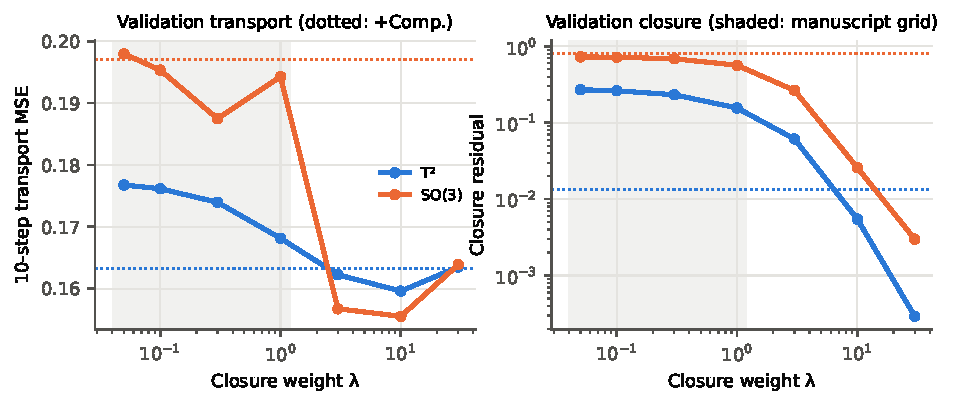
\includegraphics[width=\linewidth]{fig5_validation.pdf}
\caption{Validation sweep (seeds 5--6). The originally planned grid (shaded) does not reduce closure below
+Comp.\ (dotted); $\lambda\ge10$ does, without degrading validation transport.}\label{fig:val}
\end{figure}
\begin{figure}[h]\centering
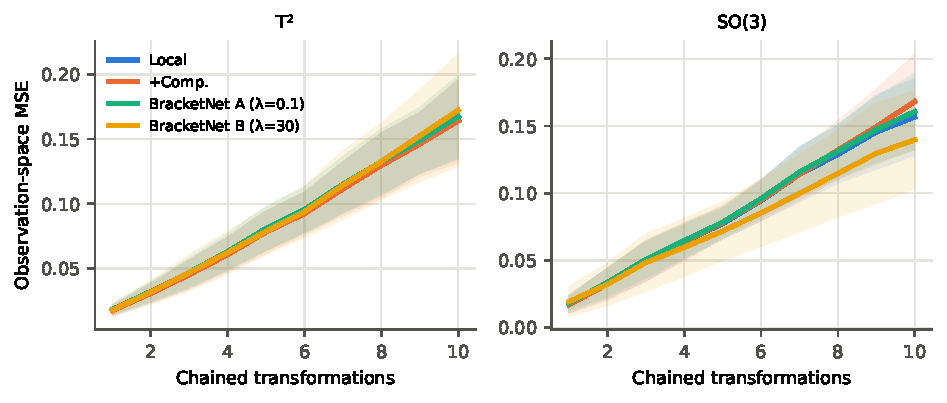
\includegraphics[width=\linewidth]{fig4_curves.pdf}
\caption{Chained transport error vs.\ path length; shading is one s.d.\ over five seeds.}\label{fig:curves}
\end{figure}
\begin{figure}[h]\centering
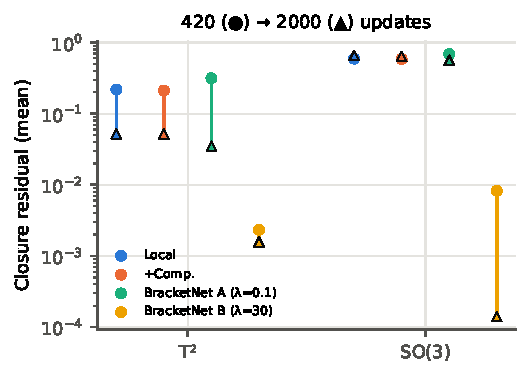
\includegraphics[width=0.5\linewidth]{fig7_budget.pdf}
\caption{Mean closure at 420 vs.\ 2,000 updates (post-hoc ablation, test seeds).}\label{fig:budget}
\end{figure}

\section{Reproducibility}
The repository contains the model and data-generation code, per-run JSON results for all 255 training runs, the
locked-hyperparameter record, figure and table scripts, the mathematical unit tests, and \texttt{run\_all.sh},
which reproduces every number in this paper.
\end{document}
